% =====================================================================
%  Betriebsanweisung Shaper Origin
%  Eigenes PDF: Betriebsanweisung_Shaper_Origin.tex, Seite in der
%  Einweisung über \BAseite. Layout: fablab-document/fablab-ba.sty
%
%  Lizenz-Hinweis: Text vollständig selbst formuliert, KEINE Passagen und
%  KEINE Abbildungen aus der Anleitung von Shaper Tools übernehmen!
%  Nur ISO-7010-Symbole und eigene Zeichnungen verwenden.
% =====================================================================
\BAsetup{
  typ=maschine,
  titel={Handgeführte CNC-Fräse Shaper Origin},
  kurztitel={Shaper Origin},
  taetigkeit={Fräsen von Konturen, Ausschnitten, Taschen und Gravuren, Fräserwechsel, Reinigen},
  nummer=BA-SO-01,
  stand=06.10.2026,                   % Datum der Freigabe
  verantwortlich={Name der verantwortlichen Person},
  bildcode={% =====================================================================
%  Kleines Symbol des Shaper Origin (von vorn) für den Kopf der
%  Betriebsanweisung (\BAsetup{bildcode=...}). Ohne zeichnungen/stil.tex
%  lauffähig. Selbst gezeichnet.
% =====================================================================
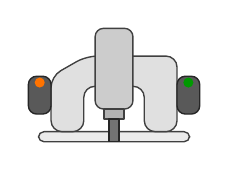
\begin{tikzpicture}[x=0.16mm, y=0.16mm, line width=0.5pt, line join=round]
  % Grundplatte
  \draw[fill=black!8, draw=black!75, rounded corners=2] (-60,0) rectangle (60,8);
  % Gehäuse mit Öffnung für die Spindel
  \draw[fill=black!12, draw=black!75, rounded corners=4] (-50,8) -- (-50,52) -- (-22,68)
    -- (50,68) -- (50,8) -- (24,8) -- (24,44) -- (-24,44) -- (-24,8) -- cycle;
  % Griffe mit Tasten
  \draw[fill=black!65, draw=black!85, rounded corners=3] (-68,22) rectangle (-50,52);
  \draw[fill=black!65, draw=black!85, rounded corners=3] (50,22) rectangle (68,52);
  \fill[orange!90!red] (-59,47) circle (4);
  \fill[green!60!black] (59,47) circle (4);
  % Spindel, Spannmutter, Fräser
  \draw[fill=black!20, draw=black!75, rounded corners=3] (-15,26) rectangle (15,90);
  \draw[fill=black!30, draw=black!75] (-8,18) rectangle (8,26);
  \draw[fill=black!55, draw=black!85] (-4,0) rectangle (4,18);
\end{tikzpicture}
},
  entwurf,
  schrift=\footnotesize,
}

\BAkopf

\BAblock{ANWENDUNGSBEREICH}{M002}{%
  \begin{itemize}
    \item Fräsen von Holz, Holzwerkstoffen und Kunststoff; Aluminium und andere Nichteisenmetalle nur nach Freigabe durch einen Betreuer.
    \item Handgeführt mit beiden Händen; die Maschine korrigiert die Position des Fräsers selbst. Werkstück immer fest auf einer gespannten Unterlage.
    \item Benutzung nur nach unterschriebener Einweisung; Anleitung des Herstellers beachten.
  \end{itemize}}

\BAblock{GEFAHREN FÜR MENSCH UND UMWELT}{W022,W024,W012}{%
  \begin{itemize}
    \item Schnittverletzungen am Fräser, der mit bis zu 26.000 Umdrehungen pro Minute läuft und nach dem Ausschalten nachläuft.
    \item Lose oder schlecht geklebte Teile werden vom Fräser erfasst und weggeschleudert.
    \item Wegfliegende Späne oder Fräserbruchstücke; Einzug von Haaren, Schmuck und loser Kleidung; Stromschlag bei angefrästem Kabel; Lärm.
    \item Gesundheitsschäden durch Staub; Hartholzstaub kann Krebs erzeugen. Brandgefahr durch überhitzte Fräser.
  \end{itemize}}

\BAblock{SCHUTZMASSNAHMEN UND VERHALTENSREGELN}{M003,M004,M017,P028}{%
  \begin{itemize}
    \item Vor jeder Benutzung Maschine, Kabel und Fräser prüfen; nur scharfe, unbeschädigte Fräser verwenden.
    \item Gehörschutz und Schutzbrille tragen, Staubmaske bei Hartholz. Anliegende Kleidung, Haare zusammenbinden. \textbf{Beim Fräsen keine Handschuhe.}
    \item Fräser nur wechseln, wenn die Spindel \textbf{vom Origin abgesteckt} ist; Spannmutter fest anziehen, danach Z-Touch.
    \item Opferplatte mit Zwingen spannen, Werkstück und \textbf{alle ausgeschnittenen Teile} mit doppelseitigem Klebeband befestigen.
    \item Immer mit Absaugung fräsen (Festool-Sauger, Stellung AUTO). Maschine mit \textbf{beiden Händen} führen.
    \item Je Durchgang höchstens halber Fräserdurchmesser tief. Fräsrichtung nach Anzeige am Bildschirm (Gegenlauf).
    \item Erst Fräser hochfahren und Spindel ausschalten, Fräser stillstehen lassen, dann Maschine abheben.
  \end{itemize}}

\BAblock{VERHALTEN BEI STÖRUNGEN UND IM GEFAHRENFALL}{W001,M006}{%
  \begin{itemize}
    \item Orange Taste drücken (Fräser fährt hoch), Spindel ausschalten, Stecker ziehen, Betreuer informieren; Schaden per Mail an \texttt{fablab-aktive@fablab.fau.de} melden.
    \item Entstehungsbrand: Maschine vom Netz trennen, löschen. \textbf{Feuerwehr: 112}
  \end{itemize}}

\BAblock{VERHALTEN BEI UNFÄLLEN – ERSTE HILFE}{E003}{%
  \begin{itemize}
    \item Spindel ausschalten, Stecker ziehen. Betreuer/Ersthelfer verständigen, Wunden versorgen.
    \item Jeden Unfall melden und im Verbandbuch eintragen.
  \end{itemize}\vspace{1.5mm}
  \textbf{Notruf: 112}\qquad FabLab: 09131\,/\,85\,28013}

\BAletzterblock{INSTANDHALTUNG, ENTSORGUNG}{M021}{%
  \begin{itemize}
    \item Wartung nur durch eingewiesene Personen mit gezogenem Stecker.
    \item Maschine nach jeder Benutzung aussaugen; Druckluft nur im Freien bzw.\ aus dem Fenster, nie auf Kamera und Bildschirm. Elektrische Prüfung nach DGUV Vorschrift 3 gemäß Prüffrist.
  \end{itemize}}
